% Fig.3 (runtime overview) is a double-column figure at the full text width;
% Fig.4 (walkthrough composite) is a single-column figure at the column width.
% The Fig.3 caption is written against the drawn content: the goal/task entry
% panel and the BINGO terminal sit outside the runtime container; inside it are
% four cooperating agents (retrieval, lead, analysis, write), the two-stage
% governance agent, and the WS/MCP/A2A/REST runtime surface; the judge/complete
% path returns to the lead agent.
\begin{figure*}[!t]
\centering
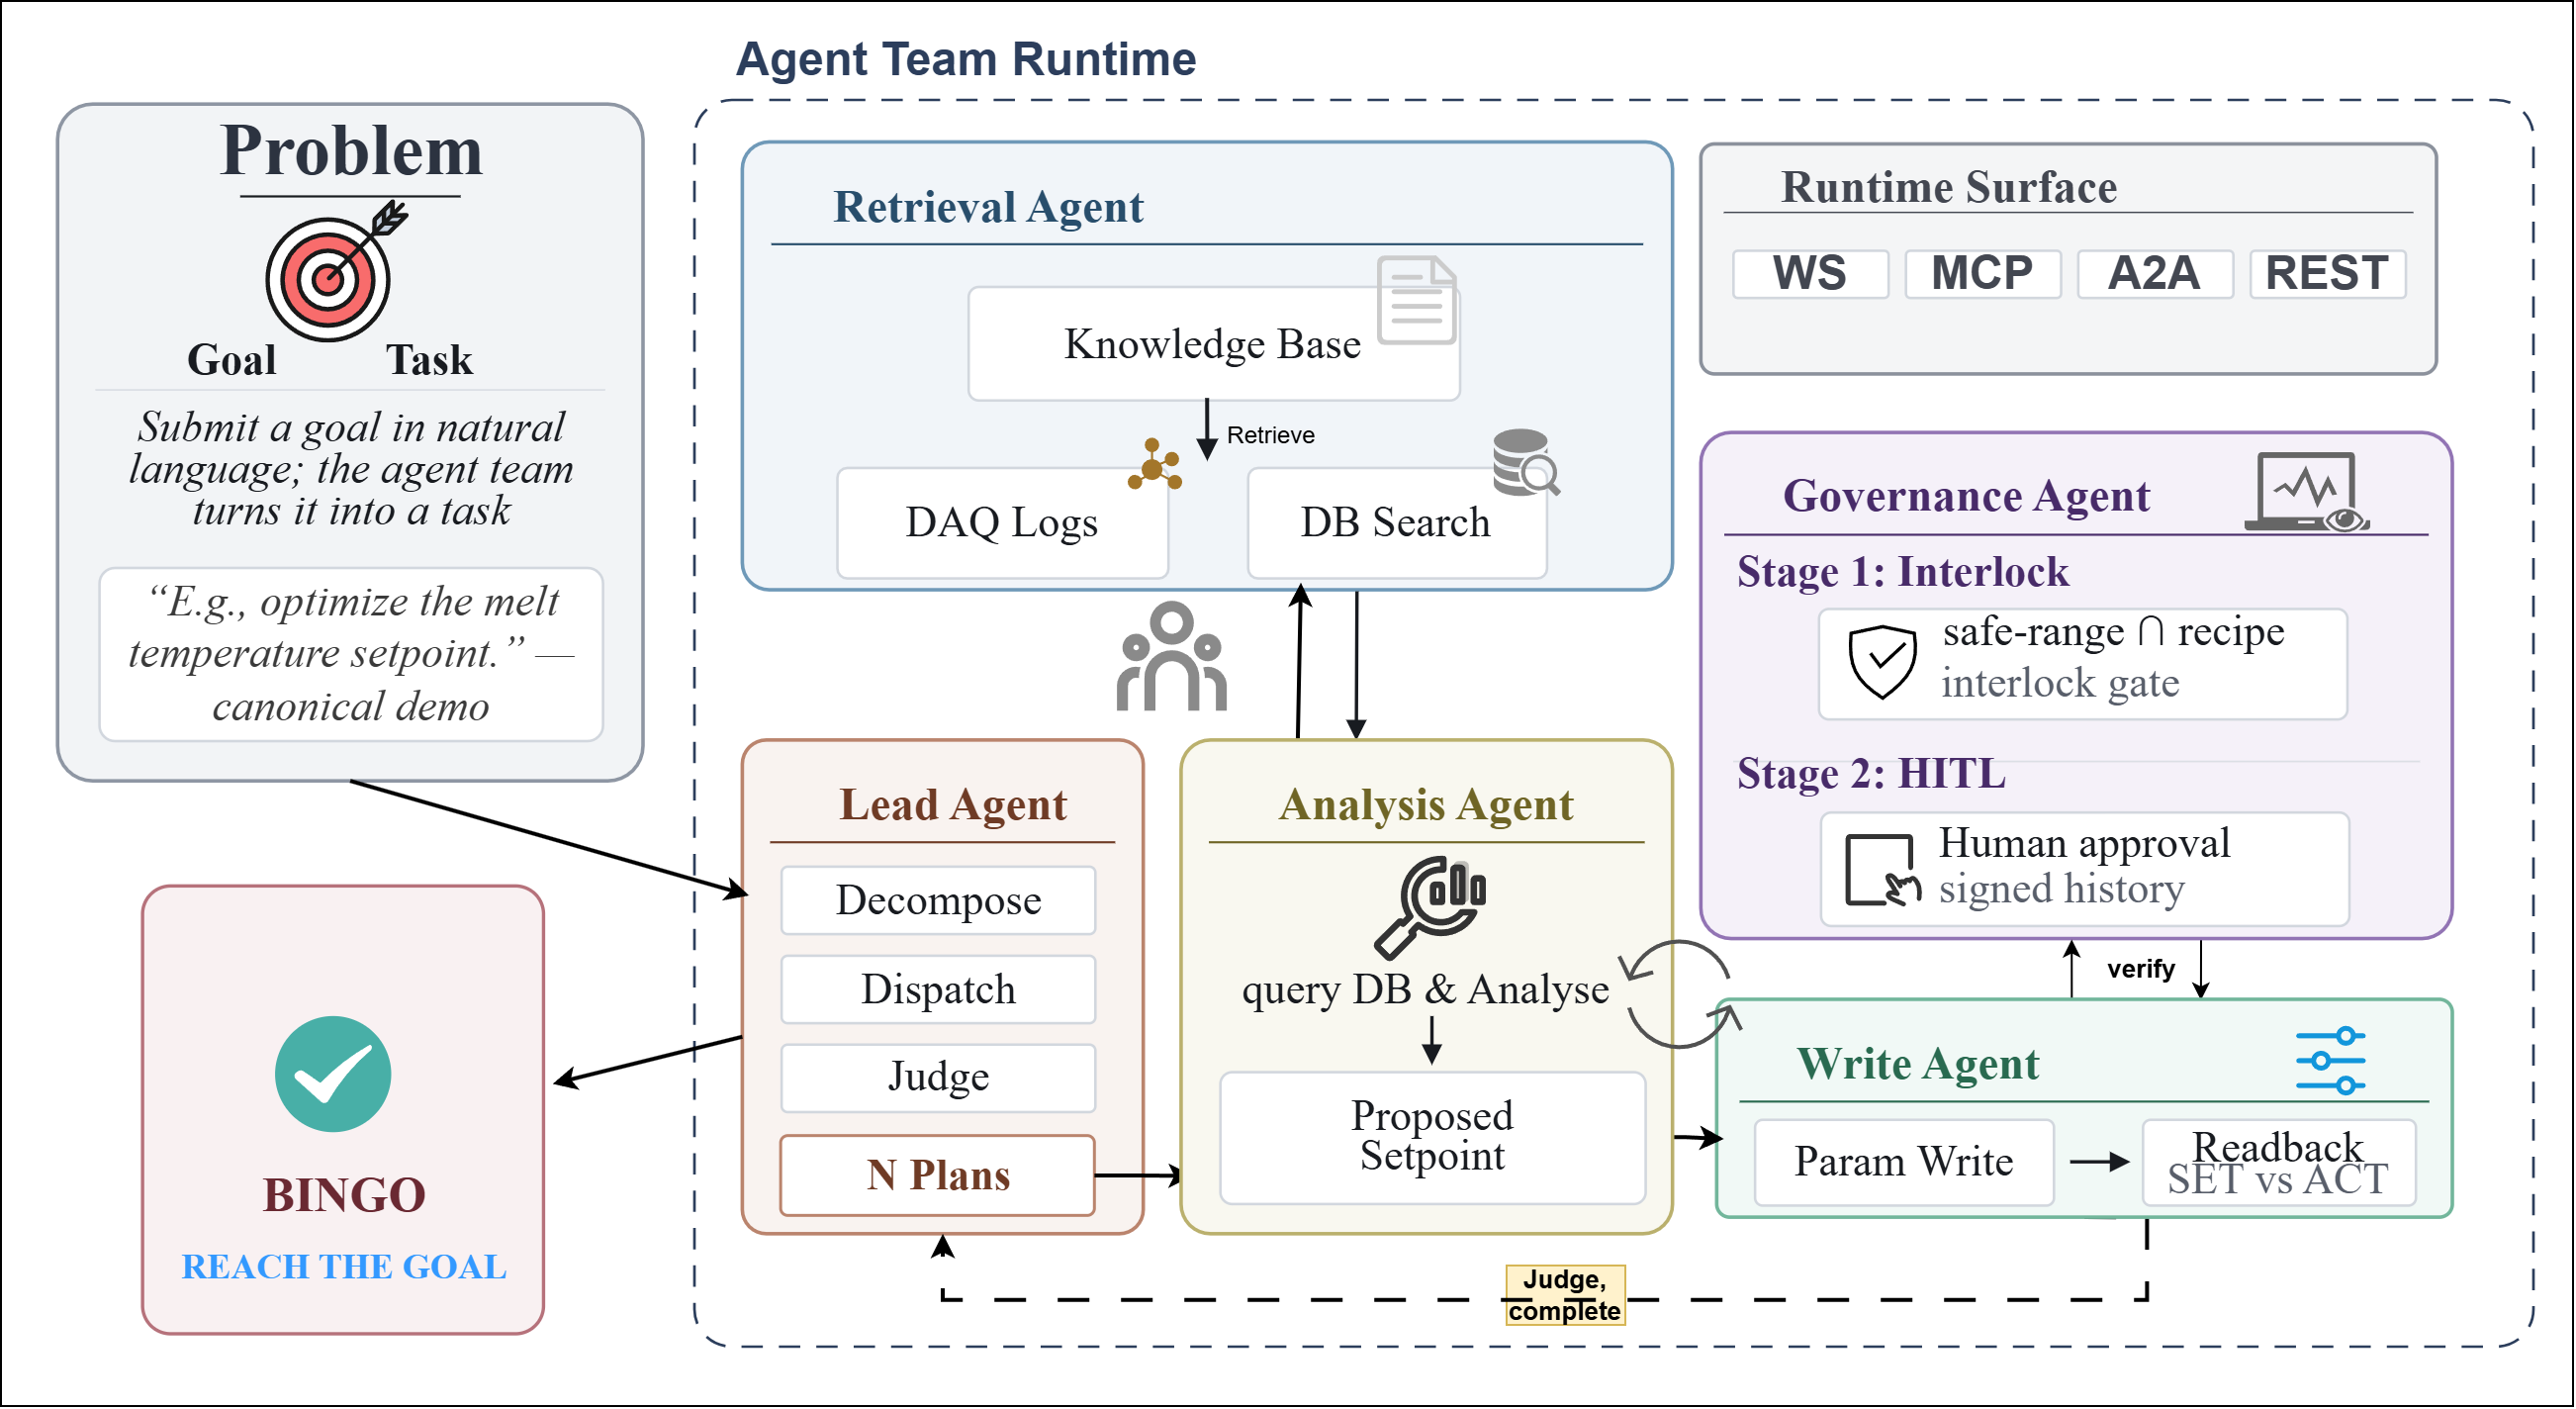
\includegraphics[width=\textwidth]{resources/aws_fig3-flat.png}
\caption{Implemented agent-team runtime. A natural-language goal enters as a
task (left); the lead agent decomposes it and dispatches one of $N$ plans; the
retrieval and analysis agents produce the proposed setpoint; the write agent
performs the write and reads the value actually present back (SET versus ACT).
The governance agent is a deterministic two-stage gate: Stage~1 intersects the
safe range with the active recipe window (drawn simplified; the implemented
admission intersects hard, baseline, product, and recipe limits, Eq.~(1)), and
Stage~2 inserts the human
approval wait on manual bindings, both journaled with actor attribution. A
judge/complete verdict returns to the lead agent, and the goal is marked
reached only along this governed path (entered over WebSocket, MCP, A2A, or
REST)---a reached goal ends the governed path, not evidence that the process
objective was met.}
\label{fig:runtime}
\end{figure*}

% Original 2x2 walkthrough composite at full column width; UI pixels authentic.
\begin{figure}[!t]
\centering
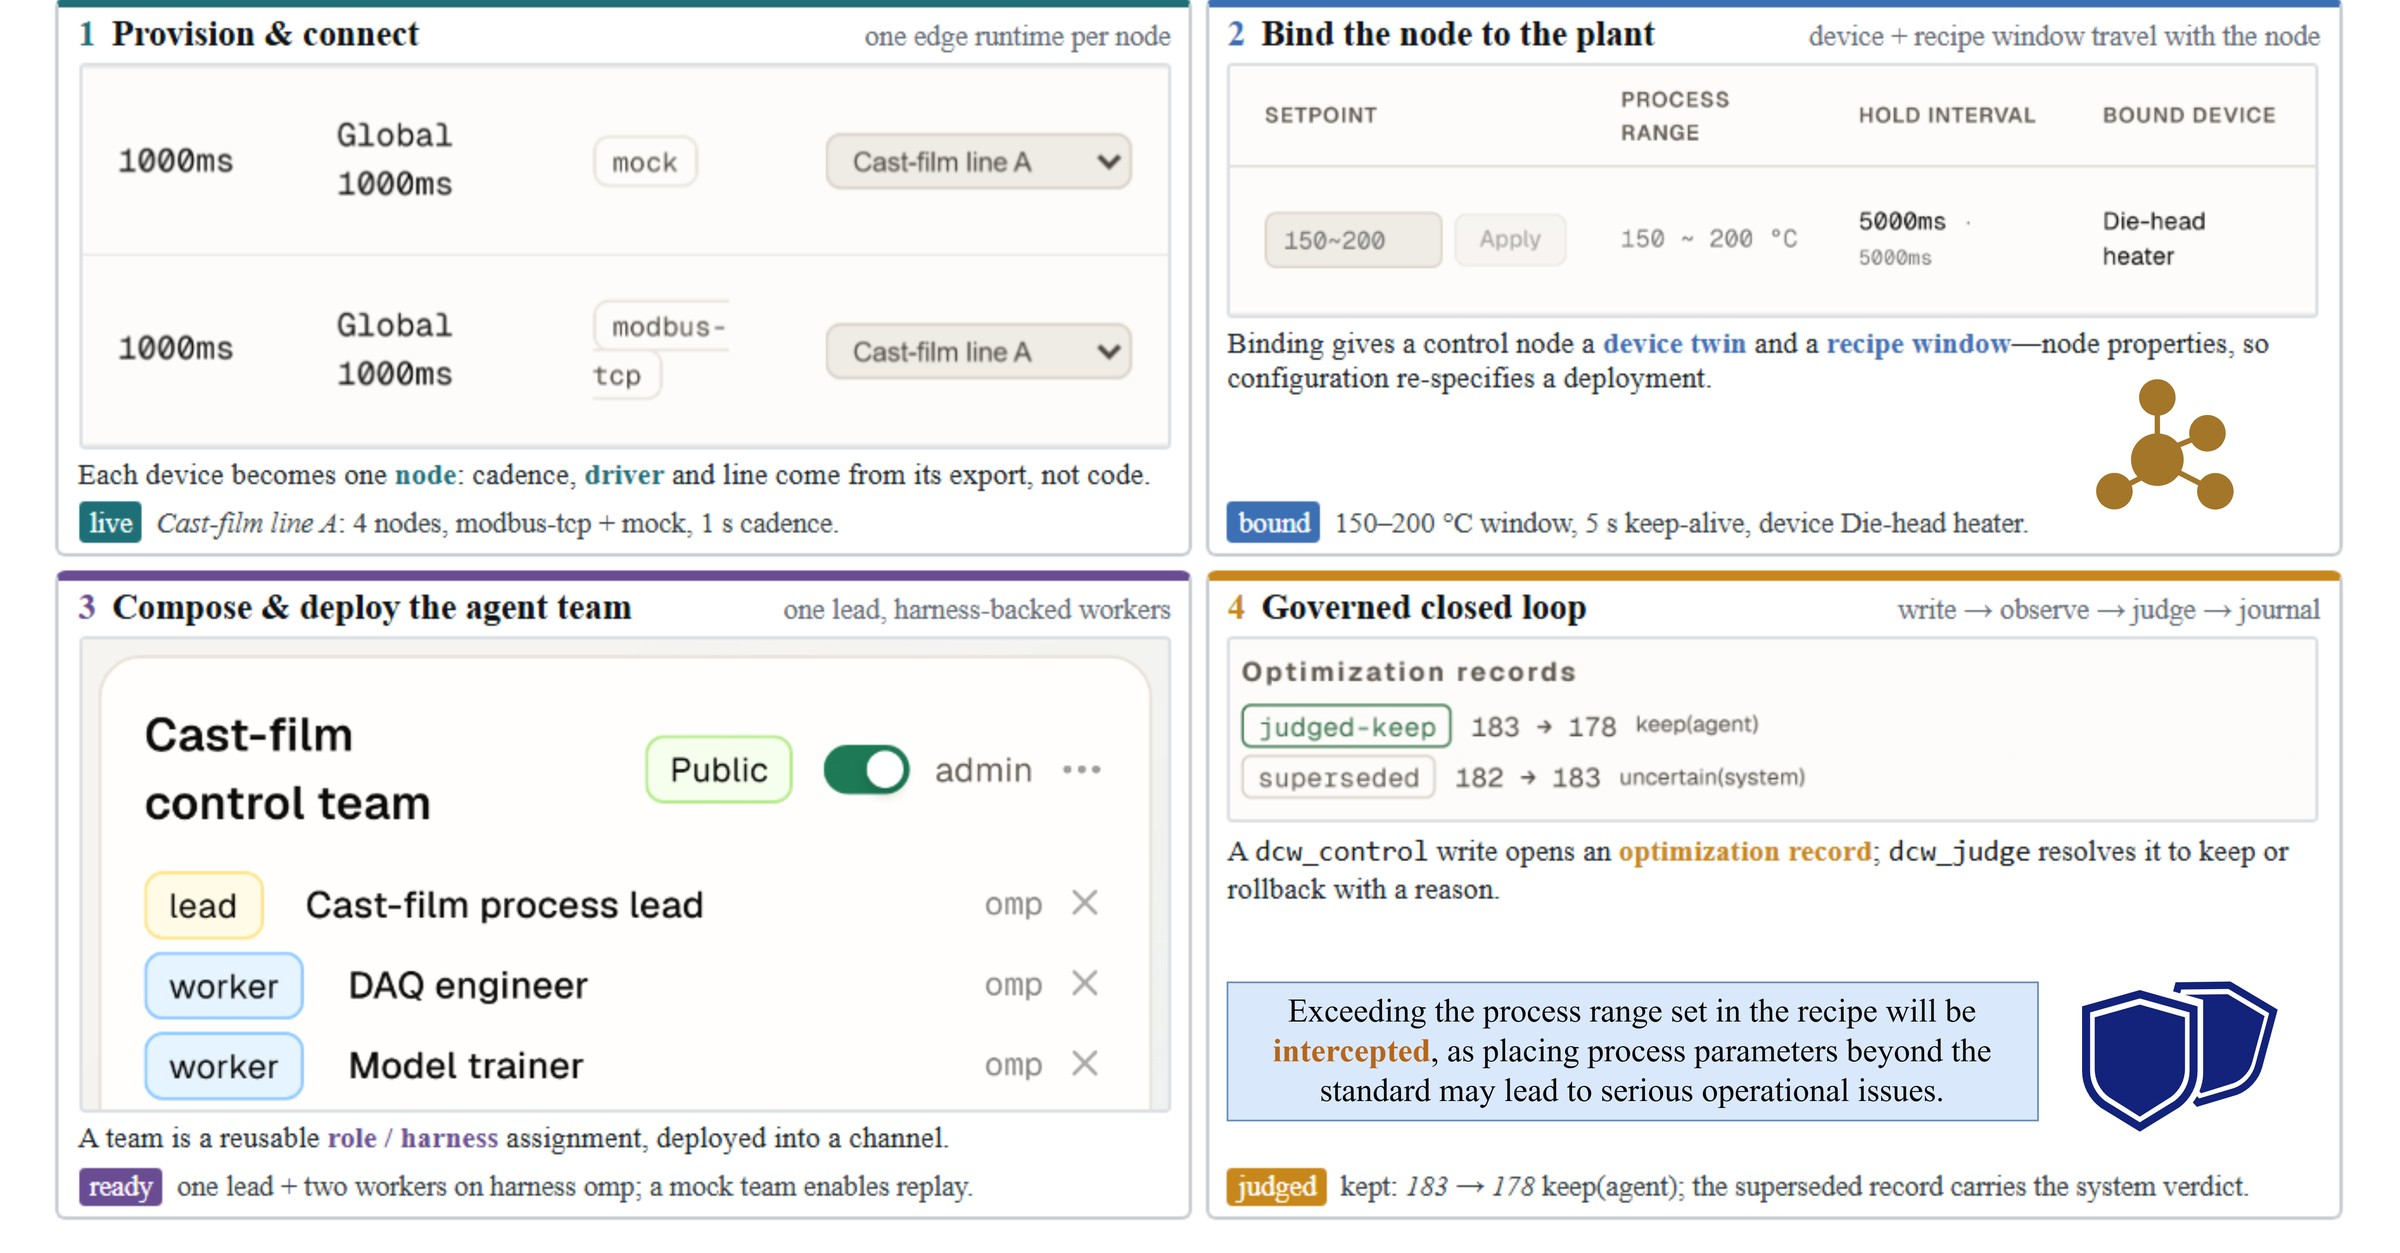
\includegraphics[width=\columnwidth]{resources/aw_working-fig4-tall-print.jpg}
\caption{The implemented path on the running operator surfaces: (1)~provisioned
nodes carry cadence, driver, and line assignment; (2)~a binding attaches the
node to its device under the active range and hold interval;
(3)~a channel deploys one lead and two workers (Fig.~\ref{fig:runtime}'s four
roles are logical and map onto lead and worker instances); (4)~a governed
closed loop opens an optimization record and stores a verdict. Running
UI/API surfaces, not benchmark outcomes.}
\label{fig:walkthrough}
\end{figure}

\section{Governed Execution Mechanisms}
\label{sec:mech}
A supervisory intervention must preserve distinctions that are often collapsed
in an agent tool call---permission to propose, admission of a value, driver
acceptance, readback, process response, a caller's verdict, and
compensation---and \system{} exposes these as separate, distinguishable
evidence states. Fig.~\ref{fig:runtime} follows one such intervention through
the implemented runtime. In it, every path that reaches the plant passes
through the same governed write---the four agents are interchangeable
participants, not control primitives---and the goal marker terminates the
workflow, which is why attainment is recorded separately from task state
throughout. The
subsections below follow that path---admission
(Section~\ref{sec:objective}), write and readback
(Section~\ref{sec:nodeexec}), observation, verdict, and compensation
(Section~\ref{sec:agentloop}), approval (Section~\ref{sec:hitl}), and the
stable plane's reuse boundary (Section~\ref{sec:rationale})---and
Fig.~\ref{fig:walkthrough} shows the path on the running operator surfaces.

\subsection{Task, Observation, and Admission}
\label{sec:objective}
The strategy receives a task and goal in production context and decides what
to propose and when to stop; the platform governs execution. Decision variables
are semantic node parameters---pressure, dosing rate, line speed, rail
width---in engineering units. Authority belongs to deployed member--node
bindings, not the channel, prompt, or task template.

Before a proposal, \texttt{daq\_query} obtains a baseline or response window
and reports freshness. For an ordinary agent setpoint request on node $n$, the
implemented admission interval is
\begin{equation}
\mathcal{I}_n(t)=\mathcal{H}_n\cap\mathcal{B}_n
                 \cap\mathcal{P}_n(t)\cap\mathcal{R}_n(t),
\label{eq:admission}
\end{equation}
where $\mathcal{H}_n$ is the hard engineering range and the remaining terms
the baseline, active-product, and active-recipe limits; missing optional
limits add no restriction. The intersection constrains submitted values---it
is not a learned feasibility region or a physical safety certificate---and
availability, binding state, and approval policy are checked separately. The
intersection bounds magnitude, not intent: in-window but adverse sequences surface
at judgment and compensation (Section~\ref{sec:scenarios} reports two).

\subsection{Semantic Write and Source-Specific Routes}
\label{sec:nodeexec}
A semantic card exposes quantity, unit, precision, range, value, freshness, and
recipe context. The controller resolves the binding and the limits; the driver
then serializes the command. Readback, where supported, closes the command
path, not the process-response path.

After a successful agent or manual write the node installs a post-write hold
window (\texttt{writeLockSeconds}, default \resWriteLock); a further
agent-origin request inside it receives HTTP 429 \texttt{WRITE\_FREQUENT}. The
lock is installed only after driver success, recipe-dispatch and rollback writes
are exempt, and zero disables it. \texttt{AW\_BENCH\_MODE=1} admits
harness-declared ablation arms on the manual route that relax the soft window
(the Stage-1 gate of Fig.~\ref{fig:runtime}), the readback check, or the
hold---the hard engineering range is never
bypassable. The hold is per node and agent-origin only: it guards a loop whose response
window may be comparable to the sampling cadence, not a rate limit on the plant.

Four governed routes---agent tools, manual writes, recipe dispatch, and
rollback compensation---reach the same driver through one admission and
journaling entry point, the hard range included; recipe dispatch adds run
context, its values validated against the recipe window when the version was
saved. Hold heartbeats are the one non-governed re-dispatch---periodic
rewrites of an already-admitted value, sharing runtime write exclusion without
re-passing admission or conferring member authority. Line
start installs active context before recipe parameters dispatch individually,
and line stop clears context and closes retained open records. These
multi-step operations are not atomic with device state.



\subsection{Observation, Judgment, and Compensation}
\label{sec:agentloop}
An accepted write opens an optimization record; the verdict tool
\texttt{dcw\_judge} records \texttt{keep}, \texttt{rollback}, or
\texttt{uncertain} plus a reason; it performs no actuation and does
not independently validate the evidence, so a scripted keep can coexist with a
missed objective. The verdict is stored with the record it closes and the
response window actually queried, so a later reader sees the evidence in front
of the caller. Verdicts are attributable---the actor and timestamp travel
with them; corrections amend the stored reason visibly rather than replacing
the verdict, and compensation opens a new record that references the one it
reverses.

Compensation is a new, separately admitted write that may fail or partially
complete; its dispatch is read-back verified, and a rollback record settles to
rolled back only once the compensating value is confirmed at the device, while
recipe rollback restores a definition, not physical PLC values. These
separations keep command status, record status, and process recovery
independently inspectable (Fig.~\ref{fig:walkthrough}).

A stored-policy backstop evaluates open records: it waits at least 120\,s,
checks at most every 30\,s, and triggers after three returned points or
averages leave the window; recovery executes only while fewer than two
retained rollback records stand on the node---a deliberate de-arm point, past
which the backstop still judges and records and defers actuation to the
record's approval policy. The cadence is neither a deadline
nor a formal run-time assurance bound.

\subsection{Human Approval Boundary}
\label{sec:hitl}
Manual bindings insert a timed approval wait before an agent setpoint or
compensation request; automatic bindings omit the wait but keep the checks.
The pending request shows member, node, value, interval, and expiry; approval
reserves neither interval nor device state, so binding and admission are
re-checked at execution. The wait fails closed: an expired request resolves as
refusal and does not actuate, with expiry and refusal recorded; duplicates are
suppressed. Selecting the approval-free mode is itself a user-side,
line-permission configuration action---agent identities hold no
binding-administration capability---so an agent cannot reclassify its own
writes as approval-free.

The decision endpoint authenticates a user but does not enforce a line-scoped
approver role, and reads, verdict recording, and some configuration changes do
not use physical-write approval: this mechanism demonstrates workflow
mediation, not segregation of duties or certified human supervision. A recipe
switch between approval and execution re-admits the value against the new
window rather than re-presenting it to the approver; the value must still
satisfy the changed interval or be rejected.

\subsection{Design Rationale and Reuse Boundary}
\label{sec:rationale}
The strategy engine is replaceable rather than trusted as a control primitive.
The stable plane keeps bindings, semantic I/O, evidence, approval, compensation,
and backstop handling, while a scenario supplies blueprint, limits, objective,
response window, and policy, confining scenario-specific work without claiming
physical portability. Two rules enforce that boundary: scenario code may
declare and configure but never execute plant I/O, so every write still passes
admission, driver dispatch, and evidence capture; and the platform never infers
a process objective, so records can be re-evaluated against a revised predicate
without rewriting history.
